\documentclass[a4paper,12pt]{article}
\usepackage[margin=1in]{geometry}

\usepackage[T2A]{fontenc}			% кодировка
\usepackage[utf8]{inputenc}			% кодировка исходного текста
\usepackage[english,russian]{babel}	% локализация и переносы
\usepackage{graphicx}                % Математика
\usepackage{amsmath,amsfonts,amssymb,amsthm,mathtools} 
\usepackage{mathtext}
\usepackage[T2A]{fontenc}
\usepackage[utf8]{inputenc}

\usepackage{wasysym}
\usepackage{multirow}
%Заговолок
\author{Бичина Марина 
группа Б04-005 1 курса ФЭФМ}
\title{}
\date{}


\begin{document} % начало документа

\begin{center}
\begin{Large}
{ Марина Б04-005, Лабораторная работа №.3.2.4}
\end{Large}
\end{center}
\paragraph{Цель работы:} 
 Исследовать свободные колебаний в электрическом колебательном контуре:
\begin{enumerate}
\itemsep0em
\item Зависимость периода свободных колебаний контура от ёмкости
\item Зависимость логарифмического декремента затухания от сопротивления
\item Определить критическое сопротивление
\item Определить добротность контура
\end{enumerate}
\paragraph{Оборудование:}
\begin{enumerate}
\itemsep0em
\item Генератор импульсов
\item Электронное реле
\item Магазин сопротивлений
\item Магазин ёмкостей
\item Катушка индуктивности
\end{enumerate}


\paragraph{Теоретическая справка:}
\paragraph{}


Основное уравнение колебательного контура 

\begin{equation}\label{ddot I}
\ddot{I} + 2\gamma\dot{I} + \omega_0^2I = 0
\end{equation}

Где $ \gamma = \dfrac{R}{2L} $ --- коэффициент затухания, $ \omega_0^2 = \dfrac{1}{LC} $ --- собственная частота контура. Решением этого уравнения являются затухающие колебания:

\begin{equation}\label{}
I = A e^{-\gamma t} \cos (\omega t - \theta)
\end{equation}

Здесь $ \omega = \sqrt{\omega_0^2 - \gamma^2} $. Можно записать решение \eqref{ddot I} и для напряжения:

\begin{equation}\label{}
U_C = U_0 \dfrac{\omega_0}{\omega} e^{-\gamma t}\cos (\omega t - \theta)
\end{equation}

В контуре с затухающими колебаниями можно использовать следующую формулу

\begin{equation}\label{}
T = \frac{T_ox}{n\cdot x_0}
\end{equation}

Режим работы контура, при котором $ \gamma = \omega_0 $, называется \textbf{критическим}. Его сопротивление равно 

\begin{equation}\label{}
R_{кр} = 2\pi\sqrt{\dfrac{L}{C}} = 2\pi\sqrt{\dfrac{\Delta Y}{\Delta X}}
\end{equation}


Добротность, потери энергии
\begin{equation}\label{Q}
Q = 2\pi \dfrac{W}{\Delta W} = \dfrac{1}{R} \sqrt{\dfrac{L}{C}} = \dfrac{\pi}{\Theta}
\end{equation}

Лог. декремент, потери амплитуды
\begin{equation}\label{theta}
\Theta = \dfrac{1}{n} \gamma T = \dfrac{1}{n} \ln \dfrac{U_k}{U_{k+n}} 
\end{equation}

Метод наименьших квадратов
\begin{equation}\label{}
y = a + bx
\end{equation}

\paragraph{Описание установки:}

\begin{center}
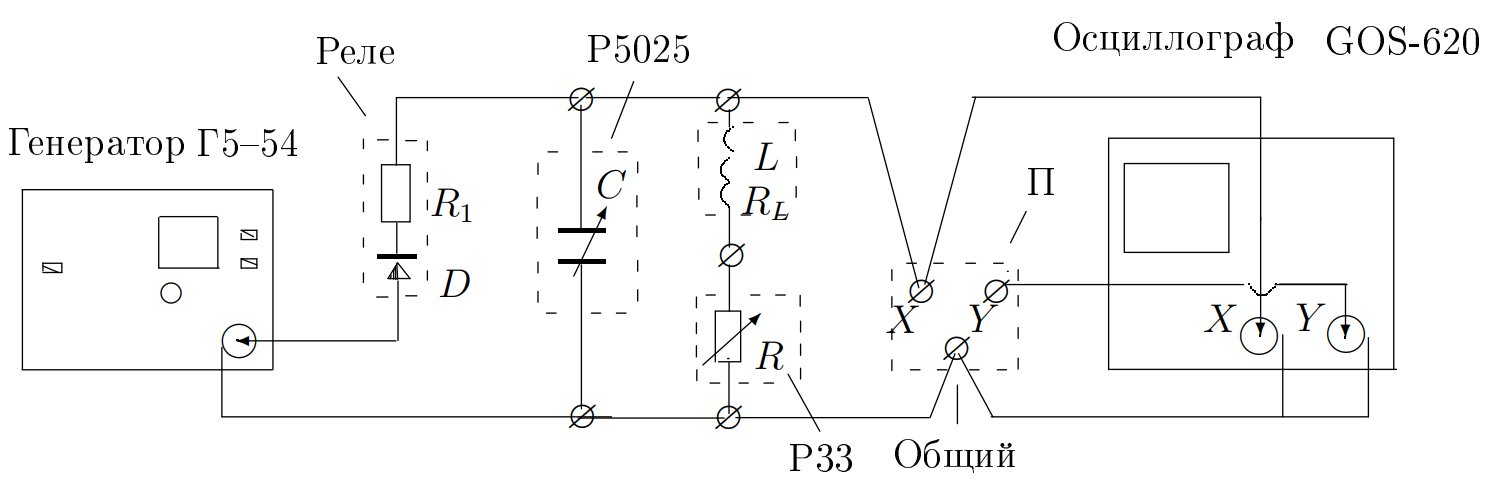
\includegraphics[scale=0.4]{setup.png} 
\end{center}
На рисунке приведена схема для исследования свободных колебаний в контуре, содержащем постоянную индуктивность $L$, переменную ёмкость $C$ и сопротивление $R$. Колебания наблюдаются на экране осциллографа.\\
Для периодического возбуждения колебаний в контуре используется генератор импульсов Г5-54. \\
Импульсы заряжают конденсатор $C$. После каждого импульса генератор отключается от колебательного контура, и в контуре возникают свободные затухающие колебания. Входное сопротивление осциллографа велико ($\approx 1$ МОм), так что его влиянием на контур можно пренебречь. 


\begin{enumerate}
\itemsep0em
\item Измерение периодов свободных колебаний:
\begin{enumerate}
\itemsep0em
\item Соберем схему, установим на магазине сопротивлений величину $R = 0$, на магазине емкостей - $C = 0.2$ мкФ.
\item Подберем частоту развертки осциллографа, измерим по шкале экрана осциллографа длительность нескольких периодов колебаний контура. Рассчитаем период свободных затухающих колебаний по формуле (4).

\begin{table}
\begin{center}
\begin{tabular}{|c|c|c|c|c|c|c|c|c|}
\hline 
С, мкФ & 0.2 & 0.3 & 0.4 & 0.5 & 0.6 & 0.7 & 0.8 & 0.9 \\ 
\hline 
$T_\text{эксп}$,мc & 0.32 & 0.4 & 0.44 & 0.5 & 0.55 & 0.58 & 0.62 & 0.67 \\ 
\hline 
$T_\text{теор}$,мc & 0.39 & 0.49 & 0.56 & 0.62 & 0.68 & 0.74 & 0.79 & 0.84 \\ 
\hline
\end{tabular} 
\caption{Таблица 1: зависимость периода от емкости}
\end{center}
\end{table}
\item Изменяя ёмкость С, проведем измерения периодов $T_\text{эксп}$ свободных колебаний при R=0. Результат занесем в таблицу 1, построим график, пользуясь МНК (ф-ла 8):

\begin{figure}
\begin{center}
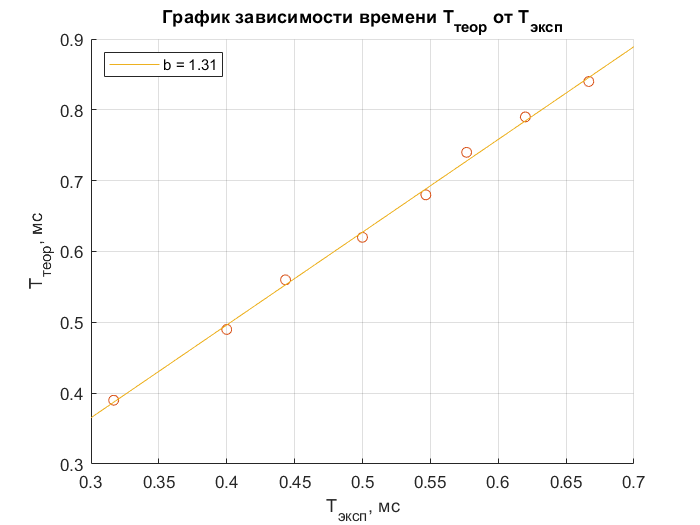
\includegraphics[scale=0.6]{graph1.png}
\end{center}
\end{figure}
Отсюда получим, что результат \textbf{отличается всего $b = 1,31$ раза}
\end{enumerate}
\item Измерение критического сопротивления и декремента затухания
\begin{enumerate}
\itemsep0em
\item Найдем логарифмический декремент затухания посредством изменения сопротивления контура

\begin{center}
\begin{tabular}{|c|c|c|c|c|}
\hline 
$\Theta$ & $R$, Ом & $R_{\sigma}$, Ом & $1/R_{\sigma}^{2} \cdot 10^{-7}$ & 1/$\Theta^2$ \\ 
\hline 
0.6 & 1100 & 1109.44 &  8.12 &  2.78  \\ 
\hline 
0.77 & 1400 & 1409.44 & 5.04 & 1.69 \\ 
\hline 
1.16 & 1700 & 1709.44 & 3.42 & 0.74 \\ 
\hline 
1.32 & 2100 & 2109.44 & 2.25 & 0.57 \\ 
\hline 
1.61 & 2400 & 2409.44 & 1.72 & 0.39 \\ 
\hline 
1.79 & 2700 & 2709.44 & 1.36 & 0.31 \\ 
\hline 
\end{tabular} 
\end{center}

\item Далее построим график зависимости $\dfrac{1}{\Theta^2}(\dfrac{1}{R^2_\text{кр}})$ 
\begin{figure}
\begin{center}
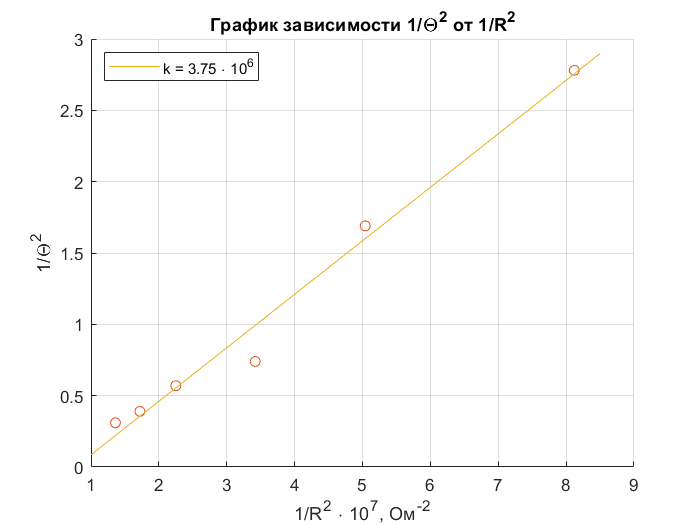
\includegraphics[scale=0.6]{graph2.png}
\end{center}
\end{figure}

По формуле (5) рассчитаем критическое сопротивление, приняв в учет то, что $\dfrac{\Delta Y}{\Delta X}=k$ при построение графика по МНК.
\begin{equation*}
R_{\text{кр}} = 2 \cdot 3.14 \cdot \sqrt{3.75} \cdot 10^3 \approx 12.161 \cdot 10^3 \text{Ом}
\end{equation*}
\item Рассчитаем погрешность  
\begin{equation*}
\varepsilon_{R} = \sqrt{\dfrac{1}{2}\varepsilon_{a} + \dfrac{1}{2}\varepsilon_{b}} \cdot 100\% \approx 8\%
\end{equation*}
\item Окончательно получим:
\begin{equation*}
R_{\text{кр}} =(12.0 \pm 1.0) \cdot 10^3 \;\; \text{Ом}
\end{equation*}
\item Далее по формуле (5) рассчитаем теоретическое критическое значение для сопротивления:
\begin{equation*}
R_{\text{кр}} = 2\pi\sqrt{\dfrac{L}{C}} = 12.649 \cdot 10^3 \;\; \text{Ом}
\end{equation*}
\item Также подберем вручную $R_{\text{кр}}$ при помощи магазина сопротивлений:
\begin{equation*}
R_{\text{кр}} =(11.010 \pm 1.0) \cdot 10^3 \;\; \text{Ом}
\end{equation*}
\end{enumerate}
\item Добротность контура
\begin{enumerate}
\itemsep0em
\item Рассчитаем добротность контура для максимального и минимального значений $\Theta$ по картине затухающих колебаний
\begin{equation*}
Q_{max} = \dfrac{\pi}{0.6} \approx 5.24
\end{equation*}
\begin{equation*}
Q_{min} = \dfrac{\pi}{1.75} \approx 1.80
\end{equation*}
\item Сравним полученные значения со значениями добротности контура, которые получаются в зависимости от характеристики контура(формула 6)
\begin{equation*}
Q_{max} \approx 5.75
\end{equation*}
\begin{equation*}
Q_{min} \approx 2.34
\end{equation*}
\item Посчитаем добротность по спирали на фазовой плоскости

\begin{center}
\begin{tabular}{|c|c|c|c|}
 \hline 
 $\Theta$ & R, Ом & $R_{\Sigma}$, Ом & Q \\ 
 \hline 
 0.81 & 1100 & 1109.44 & 3.87 \\ 
 \hline 
 0.92 & 1400 & 1409.44 & 3.43 \\ 
 \hline 
 1.16 & 1700 & 1709.44 & 2.70 \\ 
 \hline 
 1.39 & 2100 & 2109.44 & 2.27 \\ 
 \hline 
 1.60 & 2400 & 2409.44 & 1.95 \\ 
 \hline 
 1.57 & 2700 & 2709.44 & 2.00 \\ 
 \hline 
 \end{tabular}
 \end{center}
 
\end{enumerate}
\item Характеристики катушки

 Сопротивление катушки: $R_{L} = 9.44 \;$ Ом
\begin{center}
\begin{tabular}{|c|c|c|}
\hline 
$\nu$, Гц & L, мГн & R, Ом \\ 
\hline 
50 & 136 & 9.55 \\ 
\hline 
$10^3$ & 130.9 & 12.60 \\ 
\hline 
$5 \cdot 10^3$ & 131.4 & 21 \\ 
\hline 
\end{tabular}
\end{center}
\item Сводные таблицы полученных данных 

\begin{table}[h!]
	\centering
	\begin{tabular}{|c|c|c|c|}
		\hline
		\multirow{2}{*}{$L$} & \multicolumn{3}{|c|}{$R_{\text{кр}}$} \\
		\cline{2-4}
		& Теор. & Подбор & Граф.  \\
		\hline
		$ 0.2 $ Гн   & $ 12.6 \pm 1.0 $ кОм & $1.1 \pm 0.1$ кОм & 	$ 12.0 \pm 1.0 $ кОм \\
		\hline
	\end{tabular}
\end{table}

Значения критического сопротивления

\begin{table}[h!]
	\centering
	\begin{tabular}{|c|c|c|c|}
		\hline
		\multirow{2}{*}{$ R $} & \multicolumn{3}{|c|}{$ Q $} \\
		\cline{2-4}
		& Теор. & $ f(\Theta) $ & Спираль \\
		\hline
		min = 1242 Ом & $ 7,76 \pm 0,09 $ & $ 7,82 \pm 0,51 $ & $ 6,33 \pm 0,87 $ \\
		\hline
		max = 3642 Ом  & $ 2,43 \pm 0,03 $ & $ 2,47 \pm 0,27 $  & $ 2,27 \pm 0,43 $ \\
		\hline
	\end{tabular}
\end{table}

Значения добротности 

\end{enumerate}  
\paragraph{Выводы:}
\begin{enumerate}
\item Мы установили разницу между теоретическим и экспериментальным периодами колебаний. У нас эти два значения различаются в 1.3 раза, что может быть вызвано неточностью в снятии показаний или неидеальностью элементов установки.
\item Установили зависимость логарифмического декремента затухания от сопротивления 
\item Вычислили различными способами значение критического сопротивления
\item Нашли различными способами добротность контура  
\end{enumerate} 
\end{document}